\chapter{ARX-Based Mixers}
\label{appx:ARX_Mixers}
As part of the design process for the cryptosystem described in this thesis, many ARX-based mixers were analyzed before deciding to switch to a mixer based on matrix multiplication in a Galois field.
None of these ARX-based mixers were able to increase the linear and differential branch numbers from two to three, which is one of our requirements.
For completeness, we enumerate all of the mixers we analyzed here. 

One of the mixers is based on the ARX structure used in Threefish, the block cipher used within SHA-3 candidate Skein \cite{Ferguson2010_SkeinReference}. 
Another is based on the recently released lightweight block cipher Speck that was created by the National Security Agency \cite{Beaulieu2013_Speck}. 
From these ideas, more complex ARX structures were constructed and analyzed.

In all diagrams shown here, the $\mathbf{ROT}$ operation represents all possible nontrivial left and right rotations on a single word. 
Mixers corresponding to every single combination of rotations were analyzed.
The $\boxplus$ symbol denotes addition modulo $2^{16}$.
It is a nonlinear operation due to effect of the carry bit.
The $\oplus$ symbol denotes XOR, as usual.

\begin{figure}[ht]
\centering
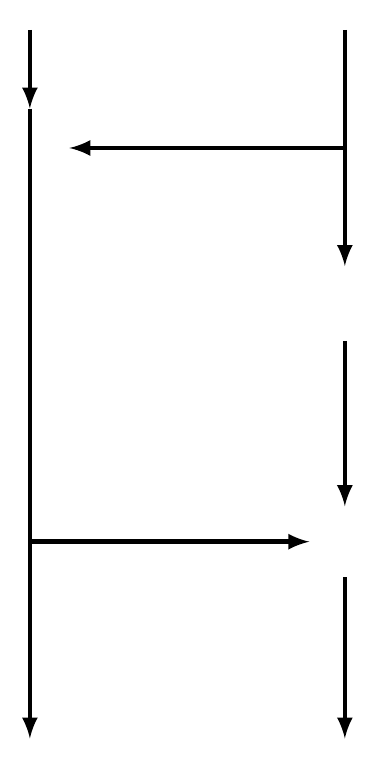
\begin{tikzpicture}[ultra thick,>=latex]
% Reference grid (temporary)
%\draw[help lines] (0,0) grid (16,16);

% Inputs A and B
\drawMixerInputs
\draw[->] (1,15) to (1,14);
\draw[->] (5,15) to (5,12);

% Modular addition
\drawAdder{0.5}{14}

% Right adder input
\draw[->] (5,13.5) to (1.5,13.5);

% Rotation
\drawRot{5}{11.5}

% XOR
\drawXOR{5}{8.5}

% XOR inputs
\draw[->] (1,8.5) to (4.55,8.5);
\draw[->] (5,11.05) to (5,8.95);

% Outputs A' and B'
\draw[->] (1,14) to (1,6);
\draw[->] (5,8.05) to (5,6);
\drawMixerOutputs{10}

\end{tikzpicture}

\caption{Candidate mixer inspired by Threefish}
\end{figure}

\begin{figure}[ht]
\centering
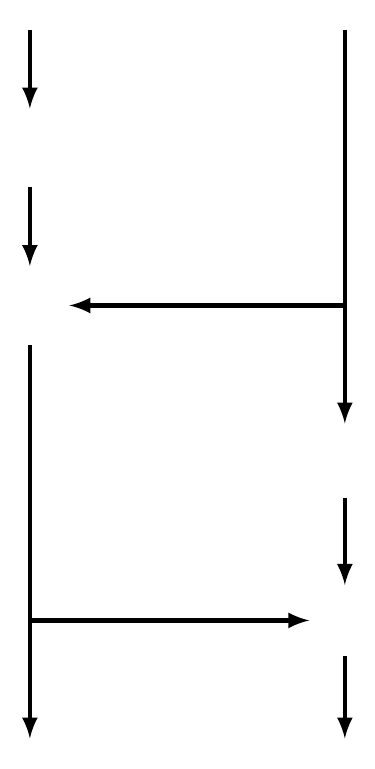
\begin{tikzpicture}[ultra thick,>=latex]
% Reference grid (temporary)
%\draw[help lines] (0,0) grid (16,16);

% Inputs A and B
\drawMixerInputs
\draw[->] (1,15) to (1,14);
\draw[->] (5,15) to (5,10);

% Rotation
\drawRot{1}{13.5}

% Modular addition
\drawAdder{0.5}{12}

% Adder inputs
\draw[->] (1,13) to (1,12);
\draw[->] (5,11.5) to (1.5,11.5);

% Rotation
\drawRot{5}{9.5}

% XOR
\drawXOR{5}{7.5}

% XOR inputs
\draw[->] (1,7.5) to (4.55,7.5);
\draw[->] (5,9.05) to (5,7.95);

% Outputs A' and B'
\draw[->] (1,11) to (1,6);
\draw[->] (5,7.05) to (5,6);
\drawMixerOutputs{10}

\end{tikzpicture}

\caption{Candidate mixer inspired by Speck}
\end{figure}

\begin{figure}[ht]
\centering
\begin{minipage}{.5\textwidth}
\centering
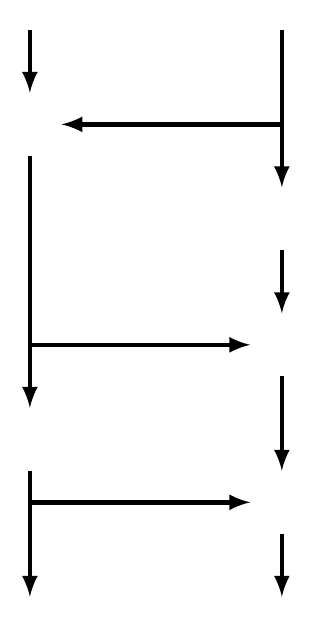
\begin{tikzpicture}[scale=0.8,ultra thick,>=latex]
% Reference grid (temporary)
%\draw[help lines] (0,0) grid (16,16);

% Inputs A and B
\drawMixerInputs
\draw[->] (1,15) to (1,14);
\draw[->] (5,15) to (5,12.5);

% Left adder 
\drawAdder{0.5}{14}
\draw[->] (5,13.5) to (1.5,13.5);

% Rotation
\drawRot{5}{12}

% Right adder
\drawAdder{4.5}{10.5}
\draw[->] (5,11.5) to (5,10.5);
\draw[->] (1,10) to (4.5,10);

% Rotation
\drawRot{1}{8.5}
\draw[->] (1,13) to (1,9);

% XOR
\drawXOR{5}{7.5}
\draw[->] (1,7.5) to (4.5,7.5);
\draw[->] (5,9.5) to (5,8);

% Outputs A' and B'
\draw[->] (1,8) to (1,6);
\draw[->] (5,7) to (5,6);
\drawMixerOutputs{10}
\end{tikzpicture}
\end{minipage}%
%
%
\begin{minipage}{.5\textwidth}
\centering
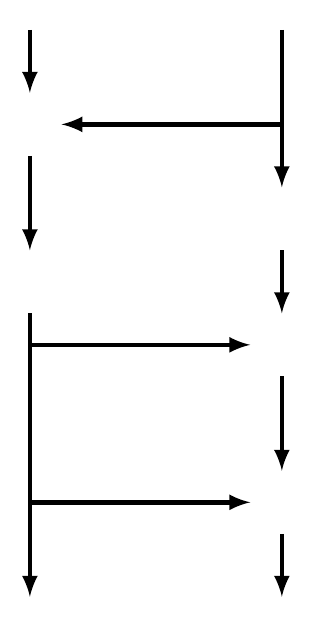
\begin{tikzpicture}[scale=0.8,ultra thick,>=latex]
% Reference grid (temporary)
%\draw[help lines] (0,0) grid (16,16);

% Inputs A and B
\drawMixerInputs
\draw[->] (1,15) to (1,14);
\draw[->] (5,15) to (5,12.5);

% Left adder 
\drawAdder{0.5}{14}
\draw[->] (5,13.5) to (1.5,13.5);

% Rotation
\drawRot{5}{12}

% Rotation
\drawRot{1}{11}
\draw[->] (1,13) to (1,11.5);

% Right adder
\drawAdder{4.5}{10.5}
\draw[->] (5,11.5) to (5,10.5);
\draw[->] (1,10) to (4.5,10);

% XOR
\drawXOR{5}{7.5}
\draw[->] (1,7.5) to (4.5,7.5);
\draw[->] (5,9.5) to (5,8);

% Outputs A' and B'
\draw[->] (1,10.5) to (1,6);
\draw[->] (5,7) to (5,6);
\drawMixerOutputs{10}
\end{tikzpicture}
\end{minipage}
%
%
\begin{minipage}{.5\textwidth}
\vspace{1cm}
\centering
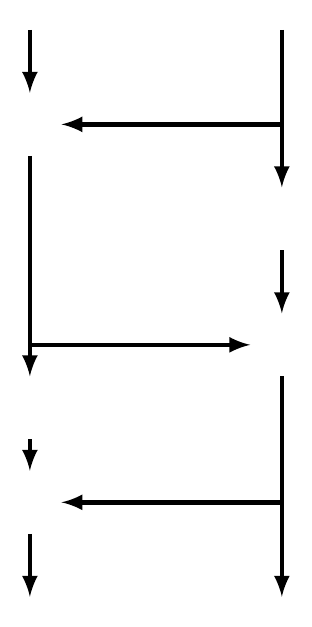
\begin{tikzpicture}[scale=0.8,ultra thick,>=latex]
% Reference grid (temporary)
%\draw[help lines] (0,0) grid (16,16);

% Inputs A and B
\drawMixerInputs
\draw[->] (1,15) to (1,14);
\draw[->] (5,15) to (5,12.5);

% Left adder 
\drawAdder{0.5}{14}
\draw[->] (5,13.5) to (1.5,13.5);

% Rotation
\drawRot{5}{12}

% Rotation
\drawRot{1}{9}
\draw[->] (1,13) to (1,9.5);

% Right adder
\drawAdder{4.5}{10.5}
\draw[->] (5,11.5) to (5,10.5);
\draw[->] (1,10) to (4.5,10);

% XOR
\drawXOR{1}{7.5}
\draw[->] (5,7.5) to (1.5,7.5);
\draw[->] (1,8.5) to (1,8);

% Outputs A' and B'
\draw[->] (1,7) to (1,6);
\draw[->] (5,9.5) to (5,6);
\drawMixerOutputs{10}
\end{tikzpicture}
\end{minipage}%
%
%
\begin{minipage}{.5\textwidth}
\vspace{1cm}
\centering
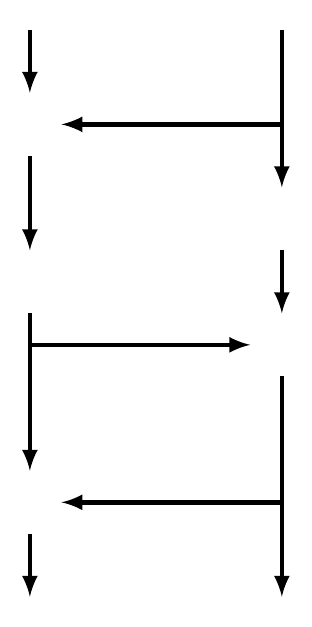
\begin{tikzpicture}[scale=0.8,ultra thick,>=latex]
% Reference grid (temporary)
%\draw[help lines] (0,0) grid (16,16);

% Inputs A and B
\drawMixerInputs
\draw[->] (1,15) to (1,14);
\draw[->] (5,15) to (5,12.5);

% Left adder 
\drawAdder{0.5}{14}
\draw[->] (5,13.5) to (1.5,13.5);

% Rotation
\drawRot{5}{12}

% Rotation
\drawRot{1}{11}
\draw[->] (1,13) to (1,11.5);

% Right adder
\drawAdder{4.5}{10.5}
\draw[->] (5,11.5) to (5,10.5);
\draw[->] (1,10) to (4.5,10);

% XOR
\drawXOR{1}{7.5}
\draw[->] (5,7.5) to (1.5,7.5);
\draw[->] (1,10.5) to (1,8);

% Outputs A' and B'
\draw[->] (1,7) to (1,6);
\draw[->] (5,9.5) to (5,6);
\drawMixerOutputs{10}
\end{tikzpicture}
\end{minipage}
%\caption{Custom candidate mixers with no initial rotation}
\caption{Custom candidate mixers}
\end{figure}

%%%%%%%%%%%%%%%%%%%%%%%%%%%%%%%%%%%%%%%

\begin{comment}
\begin{figure}[p]
\centering
\begin{minipage}{.5\textwidth}
\centering
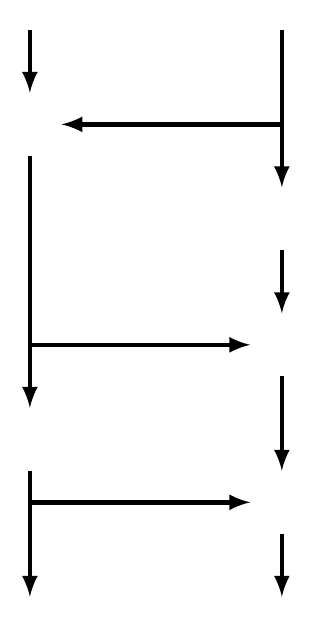
\begin{tikzpicture}[scale=0.8,ultra thick,>=latex]
% Reference grid (temporary)
%\draw[help lines] (0,0) grid (16,16);

% Inputs A and B
\drawMixerInputs
\draw[->] (1,15) to (1,14);
\draw[->] (5,15) to (5,12.5);

% Left adder 
\drawAdder{0.5}{14}
\draw[->] (5,13.5) to (1.5,13.5);

% Rotation
\drawRot{5}{12}

% Right adder
\drawAdder{4.5}{10.5}
\draw[->] (5,11.5) to (5,10.5);
\draw[->] (1,10) to (4.5,10);

% Rotation
\drawRot{1}{8.5}
\draw[->] (1,13) to (1,9);

% XOR
\drawXOR{5}{7.5}
\draw[->] (1,7.5) to (4.5,7.5);
\draw[->] (5,9.5) to (5,8);

% Outputs A' and B'
\draw[->] (1,8) to (1,6);
\draw[->] (5,7) to (5,6);
\drawMixerOutputs{10}
\end{tikzpicture}
\end{minipage}%
%
%
\begin{minipage}{.5\textwidth}
\centering
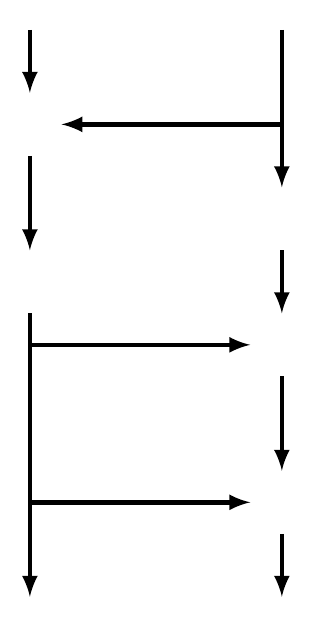
\begin{tikzpicture}[scale=0.8,ultra thick,>=latex]
% Reference grid (temporary)
%\draw[help lines] (0,0) grid (16,16);

% Inputs A and B
\drawMixerInputs
\draw[->] (1,15) to (1,14);
\draw[->] (5,15) to (5,12.5);

% Left adder 
\drawAdder{0.5}{14}
\draw[->] (5,13.5) to (1.5,13.5);

% Rotation
\drawRot{5}{12}

% Rotation
\drawRot{1}{11}
\draw[->] (1,13) to (1,11.5);

% Right adder
\drawAdder{4.5}{10.5}
\draw[->] (5,11.5) to (5,10.5);
\draw[->] (1,10) to (4.5,10);

% XOR
\drawXOR{5}{7.5}
\draw[->] (1,7.5) to (4.5,7.5);
\draw[->] (5,9.5) to (5,8);

% Outputs A' and B'
\draw[->] (1,10.5) to (1,6);
\draw[->] (5,7) to (5,6);
\drawMixerOutputs{10}
\end{tikzpicture}
\end{minipage}
%
%
\begin{minipage}{.5\textwidth}
\vspace{1cm}
\centering
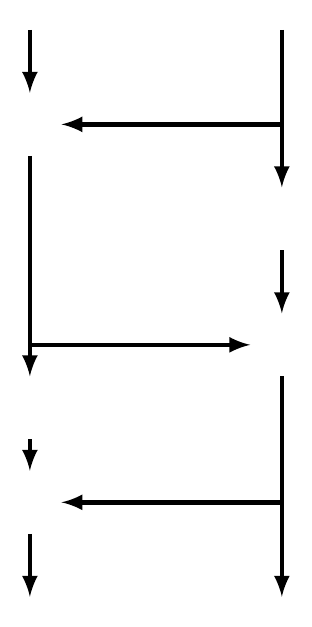
\begin{tikzpicture}[scale=0.8,ultra thick,>=latex]
% Reference grid (temporary)
%\draw[help lines] (0,0) grid (16,16);

% Inputs A and B
\drawMixerInputs
\draw[->] (1,15) to (1,14);
\draw[->] (5,15) to (5,12.5);

% Left adder 
\drawAdder{0.5}{14}
\draw[->] (5,13.5) to (1.5,13.5);

% Rotation
\drawRot{5}{12}

% Rotation
\drawRot{1}{9}
\draw[->] (1,13) to (1,9.5);

% Right adder
\drawAdder{4.5}{10.5}
\draw[->] (5,11.5) to (5,10.5);
\draw[->] (1,10) to (4.5,10);

% XOR
\drawXOR{1}{7.5}
\draw[->] (5,7.5) to (1.5,7.5);
\draw[->] (1,8.5) to (1,8);

% Outputs A' and B'
\draw[->] (1,7) to (1,6);
\draw[->] (5,9.5) to (5,6);
\drawMixerOutputs{10}
\end{tikzpicture}
\end{minipage}%
%
%
\begin{minipage}{.5\textwidth}
\vspace{1cm}
\centering
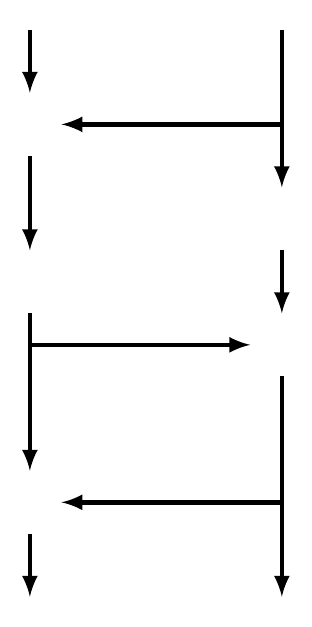
\begin{tikzpicture}[scale=0.8,ultra thick,>=latex]
% Reference grid (temporary)
%\draw[help lines] (0,0) grid (16,16);

% Inputs A and B
\drawMixerInputs
\draw[->] (1,15) to (1,14);
\draw[->] (5,15) to (5,12.5);

% Left adder 
\drawAdder{0.5}{14}
\draw[->] (5,13.5) to (1.5,13.5);

% Rotation
\drawRot{5}{12}

% Rotation
\drawRot{1}{11}
\draw[->] (1,13) to (1,11.5);

% Right adder
\drawAdder{4.5}{10.5}
\draw[->] (5,11.5) to (5,10.5);
\draw[->] (1,10) to (4.5,10);

% XOR
\drawXOR{1}{7.5}
\draw[->] (5,7.5) to (1.5,7.5);
\draw[->] (1,10.5) to (1,8);

% Outputs A' and B'
\draw[->] (1,7) to (1,6);
\draw[->] (5,9.5) to (5,6);
\drawMixerOutputs{10}
\end{tikzpicture}
\end{minipage}
\caption{Custom candiate mixers with initial rotation}
\end{figure}
\end{comment}


